% This is the central and most important section of the report. Its objective must
% be to show, with linearity and clarity, the steps that have led to the
% definition of a decision model. The description of the working hypotheses,
% confirmed or denied, can be found in this section together with the description
% of the subsequent refining processes of the models. Comparisons between
% different models (e.g. heuristics vs. optimal models) in terms of quality of
% solutions, their explainability and execution times are welcome.

% Do not attempt to describe all the code in the system, and do not include large
% pieces of code in this section, use pseudo-code where necessary. Complete source
% code should be provided separately (in Appendixes, as separated material or as a
% link to an on-line repo). Instead pick out and describe just the pieces of code
% which, for example:

% \begin{itemize}
%     \item are especially critical to the operation of the system;
%     \item you feel might be of particular interest to the reader for some reason;
%     \item  illustrate a non-standard or innovative way of implementing an algorithm, data
%           structure, etc..
% \end{itemize}

% You should also mention any unforeseen problems you encountered when implementing the
% system and how and to what extent you overcame them. Common problems are:
% difficulties involving existing software.

\subsection{Categoriche}
\textbf{Dire qualcosa sulle categoriche}

Inizialmente sono state valutate le performance di regressione dei prezzi a
partire dalle sole features categoriche in modo tale da stabilire un punto di
partenza per la successiva analisi delle features testuali, \textit{name} e
\textit{item\_description}, più complesse e computazionalmente costose.

È stato utilizzato un semplice modello composto da due layer Densi con un layer
Dropout interposto per contrastare l'overfitting.
Questo modello verrà in seguito ampliato per utilizzare anche le feature
testuali a seconda dei vari approcci.
La figura \ref{fig:modeltemplate} ne mostra un template.

\begin{figure}[h!]
	\centering
	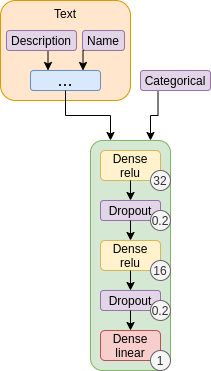
\includegraphics[
		height=8cm,
		keepaspectratio,
	]{modelTemplate.png}
	\caption{Template del modello}
	\label{fig:modeltemplate}
\end{figure}

% todo: mettere le performance nella sezione dopo
% todo: immagine del modello

% parlare di quanto tempo richiedono le 10 epoche.
% del numero dei parametri del modello.
% di quanti neuroni hanno i layers e perchè (magari fare una prova con vari
% valori bassi e aumentarli senza esagerare fino a raggiungere le performance sopra)
% parlare di qualche altro parametro? di training del modello?

\subsection{Rappresentazione del Testo}
% todo parlare della dimensionalità. di cosa è un dizionario

\subsubsection{Bag of Words}
% todo: dire qualcosa della dimensionalità di bow e tf idf?
Il modello bag-of-words è una semplice rappresentazione di testi, dove ciascuno
di essi è rappresentato come una "borsa" di parole; viene creato un vettore per
ogni documento che contiene il numero di occorrenze di ciascuna parola del
vocabolario nel documento. Questa tecnica ignora la grammatica e persino
l'ordine delle parole \cite{manning_raghavan_schutze_2008}.

\subsubsection{Tf-Idf}\label{section-tfidf} Tf-Idf (Term frequency-Inverse
document frequency) \cite{manning_raghavan_schutze_2008}, al contrario di Bag of
Words, considera l'importanza di una parola rispetto ad un documento alla luce
dell'importanza della stessa nell'intera collezione di documenti utilizzando la
frequenza in cui il termine compare prime nel documento e poi nella collezione
come mostrano le formule seguenti.% (corpus). ?
% todo: va bene parlare di documenti? vogliamo addattare più al nostro dataset?

\begin{equation}
\label{eq:tf-idf}
   Tf-Idf_{t,d} = tf_{t,d} \cdot idf_t
\end{equation}
\\
\begin{equation}
\label{eq:tf}
   tf_{t,d} = \frac{n_{t,d}}{|d|} 
\end{equation}
\\
\begin{equation}
\label{eq:idf}
   idf_{t} = \log \frac{|D|}{|\{d: t \in d\}|} 
\end{equation}
Dove in \eqref{eq:tf-idf}\eqref{eq:tf}\eqref{eq:idf} t indica il termine, d
indica il documento, D l'insieme dei documenti e le cardinalità di d e D si
riferiscono rispettivamente al numero di termini e a quello di documenti.



Per quanto riguarda il modello è stata sufficiente l'aggiunta un layer di
concatenazione in testa così da renderlo capace di accettare anche gli input
testuali nella forma di BoW.

% abbiamo dovuto aumentare i parametri rispetto alle categoriche?

\subsubsection{Word Embeddings}

Le precedenti tecniche sono semplici da realizzare, robuste e funzionali per
numerosi task. Tuttavia sono poco performanti in alcune applicazioni poiché
trattano le parole come unità atomiche, senza apprenderne relazioni complesse
ad esempio di similarità o causalità.
% nel senso che non si capisce se una parola è simile ad un altra e non si hanno
% relazioni del tipo una parola segue sempre l'altra. todo: è giusto dire
% causalità?

Con lo sviluppo delle tecniche di Machine Learning si sono diffusi i cosiddetti
\textit{word embedding} che consentono di rappresentare parole per mezzo di
vettori densi e di lunghezza fissa \cite{almeida2019word}, fornendo di
conseguenza una rappresentazione più efficiente rispetto alla \textit{Bag of
words} sparsa e dimensionalmente più costosa.
% todo: meglio dire prima che la bow è sparsa ?

Inoltre questi vettori sono in grado di apprendere la similarità tra parole così
come regole semantiche o sintattiche, permettendo anche operazioni algebriche
\cite{mikolov2013efficient}.
% dobbiamo sapere cosa significa semantico e sintattico

% word embedding di keras
\subsubsection{Keras Embedding Layer}

Keras fornisce un implementazione di embedding sotto la forma di layer neurale
e ne rende quindi possibile l'addestramento insieme al resto del modello;
altrimenti permette di fissare il valore dei pesi semplificando l'integrazione
con modelli pre-allenati.

% Nel modello è stata utilizzata l'implementazione di word embedding fornita da
% Keras sotto forma di layer. La sua dimensionalità è stata impostata a 50 e to
% be continued... todo dire ciò in qualche modo


\subsubsection{GLOVE}
GLOVE (Global Vectors) è un modello di apprendimento non supervisionato allenato
a partire dalle statistiche globali di co-occorrenza delle varie parole
\cite{pennington2014glove}. Sono inoltre disponibili modelli GLOVE
pre-addestrati; seguono quelli utilizzati nel progetto.
\begin{itemize}
	\item Wikipedia 2014 + Gigaword 5: allenato su 6 miliardi di parole e con un
	vocabolario di 400 mila parole;
	\item Common Crawl: allenato su 840 miliardi di parole e con un vocabolario
	di 2.2 milioni di parole (il più grande tra i modelli GLOVE pre-addrestrati);
\end{itemize}

\subsection{modello}\label{Modello}
Nella realizzazione di questo progetto sono stati utilizzati due modelli
principali che trattano le tecniche di rappresentazione utilizzate ed  entrambi
i modelli condividono la seguente struttura:
\begin{itemize}
	\item \textbf{Concatenate layer}: concatena gli input in un singolo tensore;
	\item \textbf{Dropout layer}: per escludere una frazione dell'input e il fattore utilizzato è 0.2;
	\item \textbf{Dense layer}: composto da 32 neuroni e come funzione di attivazione usa la Relu;
	\item \textbf{Dropout layer}: utilizza un fattore di 0.2;
	\item \textbf{Dense layer}: composto da 16 neuroni e come funzione di attivazione usa la Relu;
	\item \textbf{Dense layer}: rappresenta il layer di output ed è composto da un neurone con funzione di attivazione lineare poiché il task è una regressione;
\end{itemize}
\subsubsection{Word Embeddins}
Il modello principale utilizzato per i Word Embeddings (sia pretrainati che non)
tratta i seguenti input differentemente: descrizione del prodotto, variabili
categoriche del prodotto (nome, categorie, brand, shipping e condizione) e nome
del prodotto.
La descrizione e il nome vengono rappresentati sotto forma di interi, dove ogni
intero rappresenta l'indice di un token in un dizionario.
Le variabili categoriche che non prevedevano un valore intero sono state
convertite in valori interi.
La descrizione prevede un layer di embedding, il quale crea la rappresentazione
vettoriale densa delle parole e nel caso di GLOVE i pesi utilizzati non sono
apprendibili in quanto vengono utilizzati quelli pretrainati.
Successivamente sono stati utilizzati due layer LSTM Bidirezionali per trattare
questo input e il primo layer prevede 16 celle LSTM e un fattore di dropout di
0.2, mentre il secondo prevede 8 celle LSTM e anch'esso utilizza un fattore di
dropout di 0.2.
Infine sul campo descrizione viene utilizzato un GlobalMaxPooling1D per il sotto
campionamento in una rappresentazione più compatta.
Anche il nome viene trattato tramite un layer di embedding (anche qui con GLOVE
vengono utilizzati i pesi pretrainati), successivamente è stato utilizzato un
layer di LSTM Bidirezionale con 12 celle e un fattore di dropout di 0.2; infine
è stato utilizzato anche qui il GlobalMaxPooling1D.
Sulle variabili categoriche non sono state effettuate altre operazioni.
I tre nuovi input ottenuti vengono passati nel layer di concatenazione e quindi
nella struttura spiegata precedentemente all'inizio della sezione \ref{Modello}.

Nel modello sono stati utilizzati layers di RNN per trattare i dati non
strutturati, poiché sono ottimi per l'elaborazione di dati sequenziali e nei
testi per assegnare un'interpretazione corretta la relazione delle parole è
molto importante. Infatti, le RNN elaborano una sequenza di input un elemento
alla volta, mantenendo in "memoria" informazioni sugli elementi passati della
sequenza \cite{liang2017text}.

\subsubsection{Transformers}
% diremo che il trasform supera lstm. todo pro-cons lstm: tipo memoria,...
Il Transformer è un'architettura proposta nel 2017 che si contrappone alle RNN
evitando quindi la ricorrenza e utilizzando esclusivamente un meccanismo di
\textit{attention} per rappresentare i rapporti di dipendenza di input e output.
Si basa su di una struttura \textit{encoder-decoder} dove l'encoder fornisce al
decoder una rappresentazione dell'input ed in seguito il decoder fornisce una
frase in output \cite{vaswani2017attention}.

% BERT’s model architecture is a multi-layer bidirectional Transformer encoder
% based on the original implementation

Una delle più note architetture basata sul concetto di Transformer è
\textbf{BERT}, ovvero \textit{Bidirectional Encoder Representations from
Transformers}; si tratta di un transformer multi-layer bidirezionale, cioè in
grado di apprendere relazioni di dipendenza di un dato elemento dell'input sia
rispetto agli input precedenti che ai successivi, che si basa esclusivamente su
di moduli encoder. È stato introdotto con il fine di fornire un modello
pre-allenato semplicemente adattabile ad un vasto range di applicazioni tramite
\textit{fine-tuning}. Tuttavia anche gli approcci \textit{feature-based} basati
su BERT risultano efficaci \cite{devlin2018bert}.

In questo progetto BERT è stato utilizzato con quest'ultimo approccio
feature-based occupando effettivamente nel modello la stessa posizione dedicata
agli embedding per entrambi i campi nome e descrizione; il resto del modello è
pressochè invariato rispetto a quello precedentemente descritto, ovvero a
seguito di BERT troviamo fino a due layer LSTM bidirezionali (uno per il nome),
un GlobalMaxPooling1D e gli ultimi due layer Densi entrambi preceduti da un
dropout.

\subsubsection{Training e valutazione}

\subsubsection{Dataset split}

Al fine di valutare i vari modelli più correttamente possibile il dataset è
stato suddiviso in \textit{training-set}, \textit{validation-set} e
\textit{test-set}. Quindi il training è stato usato per l'allenamento, il
validation per accertarsi che il modello non sia propenso all'overfitting ed il
test per la valutazione finale.

\subsubsection{Valutazione dell'errore}
% loss e metriche

Per quanto riguarda le performance in termini di errore la funzione di
\textit{loss} utilizzata in fase di training è il \textit{Root Mean Squared
Logaritmic Error (RMSLE)}, in quanto è la misura scelta dalla Kaggle challenge
per confrontare le performance dei vari partecipanti. Inoltre essa risulta
adeguata al problema considerando il vasto intervallo dei valori dei prezzi.

Di seguito la definizione e alcune osservazioni su di RMSLE e su un'ulteriore
metrica utilizzata, il \textit{Mean Absolute Error (MAE)},
che fornisce una più immediata comprensione rispetto al RMSLE. \\
Mean Absolute Error (MAE):
\begin{equation}
    \frac{1}{n} \sum_{i=1}^{n} | y_i - \hat{y_i} |
\end{equation}
\\
Mean Squared Logarithmic Error (MSLE): essendo calcolato a partire da un
rapporto riflette l'errore relativo e di conseguenza risulta efficace laddove i
valore assoluti presentano variazioni considerevoli.
\begin{equation}
    \frac{1}{n}
        \sum_{i=1}^{n}
            ( \log(y_i+1) - \log(\hat{y_i}+1) )^2
    =
    \frac{1}{n}
        \sum_{i=1}^{n}
            \log^2(\frac{y_i+1}{\hat{y_i}+1})
\end{equation}
\\
Root Mean Squared Logarithmic Error (RMSLE): la radice dell'MSLE.
\begin{equation}
    \sqrt{ 
        \frac{1}{n}
            \sum_{i=1}^{n}
                ( \log(y_i+1) - \log(\hat{y_i}+1) )^2
    }
\end{equation}

% dire da qualche parte qualche altra valutaione: e.g. la computazione richiesta
% dai vari approcci

\subsubsection{Valutazione dei costi computazionali}

Il numero dei parametri allenabili dei vari modelli sono stati annotati insieme
al tempo richiesto per l'esecuzione di 10 epoche di train sulla piattaforma
\textit{Google Colab} abilitando l'accelerazione hardware GPU.


\subsection{TODO}

adam, earlystopping, batchsize, learning rate.
